\section{Scope of the system}

As an example, the system might have the following components. Some components might be reused from existing open-source projects, while others might be developed from scratch.

\begin{itemize}
    \item A git server, behind a ssh server
    \item A git-lfs server, behind a reverse proxy
    \item A storage server
    \item An authentication wrapper
    \item An implementation of the git-lfs-authenticate command
    \item A modifiable configuration of repos and user
\end{itemize}

We can draft in figure \ref{fig:architecture} a possible architecture of the system.

\begin{figure}[h]
    \centering
    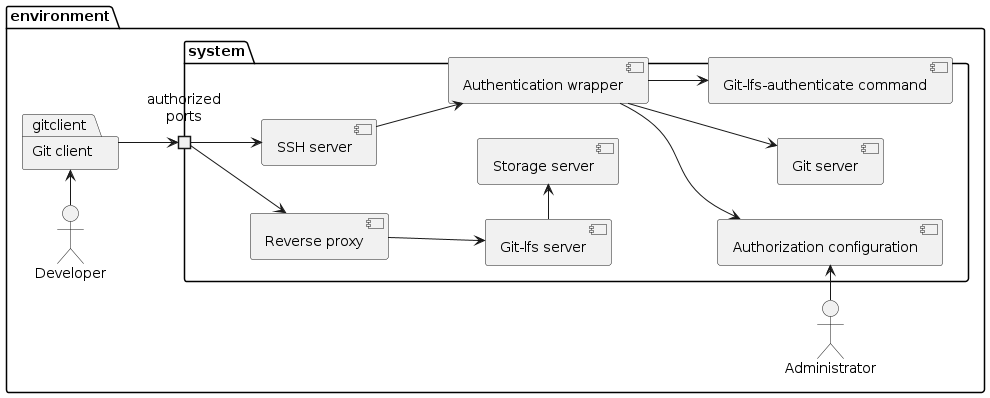
\includegraphics[width=\textwidth]{iteration_01/diagrams/context.png}
    \caption{A possible simple architecture of the system, drawing boundaries between the system and the external components}
    \label{fig:architecture}
\end{figure}

The fist assumption that we will make it that the git client is not part of the system, nor is the administrator system. However, interfaces to these systems shall be provided.

Other organization might only use some components, and make other external components of the system. For example, the storage server will be considered part of the system for this project, but it should be easy to replace it with another storage server, so good interfaces will be provided.
